\documentclass[11pt]{article}
\usepackage[margin=1in]{geometry}
\usepackage{graphicx}
\usepackage{siunitx}
\usepackage{amsmath}
\usepackage{float}
\usepackage{caption}
\usepackage{circuitikz}
\usepackage{hyperref}
\usepackage{booktabs}

\title{Lab 6: RC Oscillator Circuits}
\author{Jason Jain \\
        Oregon State University, Department of Physics \\
        Electronics Laboratory}
\date{\today}

\graphicspath{{output/}{./}{./output/}{lab-6/output/}{data/}}

\begin{document}

\maketitle


\begin{abstract}
We construct an RC relaxation oscillator using an LM358 op-amp configured as a voltage comparator with positive and negative feedback. The circuit converts a \qty{+5}{\volt} DC supply into a square-wave output whose frequency is set by the RC time constant. We measure the oscillation period for two capacitance values ($C=\qty{75}{\nano\farad}$ and $C=\qty{9.3}{\micro\farad}$) at $R=\qty{3.2}{\kilo\ohm}$ and compare to the theoretical prediction $T=2RC\ln 3$. Measured frequencies agree with theory to within $5\%$, confirming the model.
\end{abstract}


\section{Introduction}

Op-amps are powerful and fundamental electrical components used widely in modern technology. An op-amp takes two voltage inputs $V_+, \ V_-$ and performes a comparison operation; the difference $V_+ - V_-$ is then amplified by a gain factor $G_0$.  In a closed loop configuration, like the one we work with in this lab, the op-amp will constantly try to equalize $V_+, \ V_-$ and minimize the input current $I_\mathrm{in}$. To explore the applications of op-amps, we build a simple RC oscillator circuit that generates a square-wave AC current from a simple $\qty{+5}{\volt}$ DC input. By adjusting our resistance and capacitance, we can adjust the frequency of the square wave.


\section{Theory}


\begin{figure}[H]
        \centering
        \begin{circuitikz}[american, scale=0.7, transform shape]
                \draw (0,0) node[op amp] (opamp) {}
                (opamp.+) node[left] {}
                (opamp.-) node[left] {};
                \draw (opamp.out)
                to[short, -*] ++(0.5,0) coordinate(out1)
                to[short, -*] ++(1,0) coordinate(out2);
                \draw (out2)
                to[led] ++(0,-2) coordinate (led)
                to[R, l=$\qty{100}{\ohm}$] ++(0,-1.5) node[ground]{};
                \draw (out2)
                to[loudspeaker] ++(0,2) node[ground, rotate=180]{};

                % loop back
                \draw (opamp.+)
                to[short, -] (-1.5, -0.5) |- (-1.5, -2) coordinate(o_plus1)
                to[R, l=$\qty{10}{\kilo\ohm}$, *-] +(3, 0) -| (out1);
                \draw (o_plus1)
                to[R, l=$\qty{10}{\kilo\ohm}$, *-] ++(-2.5, 0) -| (-5,-3);

                % potentiometer
                \draw (1,2) coordinate (p_start)
                to[pR, l_=$\qty{10}{\kilo\ohm}$, name=P, *-*] (-1.5,2) coordinate (p_end);
                \draw (P.wiper) to[short]  ++(1, 0) -| (out1);
                \draw (opamp.-)
                to[short, -] (-1.5, 0.5) |- (p_end)
                to[C, l=$C$] (-4,2)
                to[short, -*] (-5,2) coordinate (tp);
                \node[above left] at (tp) {TP (\qty{2}{\volt})};

                % voltage divider 
                \draw (-7,-3) node[vcc]{+5V}
                to[R, l_=$\qty{330}{\ohm}$, -*] (-5,-3) coordinate(v_divider)
                to[R, l_=$\qty{220}{\ohm}$, *-] ++(2,0) node[ground]{};
                \draw (v_divider) to[short] (tp);
        \end{circuitikz}
        \caption{RC relaxation oscillator circuit. The op-amp acts as a comparator with positive feedback (two \qty{10}{\kilo\ohm} resistors) setting the switching thresholds and negative feedback (potentiometer $R$ and capacitor $C$) setting the RC time constant. The voltage divider (\qty{330}{\ohm}, \qty{220}{\ohm}) biases the circuit at \qty{2}{\volt}. The LED and speaker are driven from the output.}
        \label{fig:circuit}
\end{figure}


Given two resistors $R_1, \ R_2$, a voltage divider sets a threshold voltage, weighted by each resistance. 

\begin{equation}
  \label{eq:vdivider}
  V_{\text{divider}} =   \frac{V_\mathrm{in} R_2}{R_1 + R_2}
\end{equation}

Circuit~\ref{fig:circuit} takes input power $\qty{+5}{\volt}$ and feeds it into a voltage divider (lower left) with $R_1=\qty{220}{\volt}, \ R_2=\qty{330}{\volt}$. By Eq~\eqref{eq:vdivider}, the reference voltage is set to ${(5) (330)} / {550}=\qty{2}{\volt}$, which we measure at our test point (TP, top left). 

The positive feedback ($V_+$) path is stabilized by another voltage divider with $R_1=R_2=\qty{10}{\kilo\ohm}$, for a reference voltage ${(2) (10000)} / {20000}=\qty{1}{\volt}$ This will become the reference voltage that the op-amp will use to equalize the negative input ($V_-$), which is connected to a capacitor $C$ and a potentiometer. Once the capacitor is charged beyond the reference voltage, this equalization will force a discharge cycle, and vice-verse once it is discharged below the reference voltage. This cycle repeats indefinitely, creating a square wave. 

\subsection{Oscillation period}

For a symmetric threshold (equal feedback resistors $R_1 = R_2$), the capacitor charges between $V_{\text{ref}} - \Delta V$ and $V_{\text{ref}} + \Delta V$ where $\Delta V = V_{\text{sat}}/3$ for the $1/2$ divider ratio. Solving the RC charging equation for each half-cycle gives a half-period of $\tau_{\text{half}} = RC\ln 3$, so the full period is
\begin{equation}
  \label{eq:period}
  T = 2RC\ln 3
\end{equation}
and the oscillation frequency is $f = 1/T$.

The LED and speaker are driven from the output node. The \qty{100}{\ohm} resistor in series with the LED limits current to a safe level. The LED blinks at the oscillation frequency, and the speaker produces an audible tone when $f$ is in the audio range.



\section{Experimental Procedure}

We assembled Circuit~\ref{fig:circuit} on a breadboard (Figure~\ref{fig:breadboard}) and powered it with a \qty{+5}{\volt} DC supply. The potentiometer was set to $R = \qty{3.2}{\kilo\ohm}$ (measured with a multimeter). We tested two capacitor values: $C = \qty{75}{\nano\farad}$ and $C = \qty{9.3}{\micro\farad}$.

For each configuration, we recorded the op-amp output (Pin 1) and the test probe (TP) waveforms on different channels of our oscilloscope. We also counted LED blinks and listened to the speaker output to qualitatively verify the oscillation frequency. 


A photograph of the LED in operation is shown in Figure~\ref{fig:breadboard}.

% PLACEHOLDER: replace with photo of LED on if available
\begin{figure}[H]
        \centering
        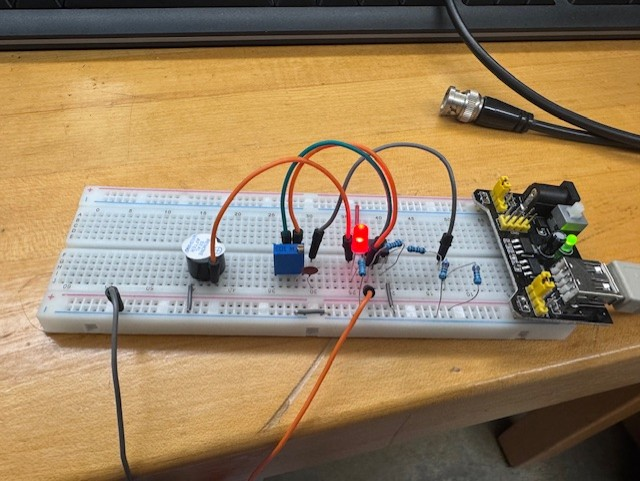
\includegraphics[width=0.5\columnwidth]{data/circuit.jpg}
        \caption{Breadboard implementation of Circuit~\ref{fig:circuit} with the LED illuminated during the high output phase.}
        \label{fig:breadboard}
\end{figure}


\section{Results and Discussion}

\subsection{Oscilloscope traces}

Figures~\ref{fig:osc_75nF} and~\ref{fig:osc_9uF} show the recorded output and probe waveforms for the two capacitance values at $R = \qty{3.2}{\kilo\ohm}$. For $C = \qty{9.3}{\micro\farad}$, $R = \qty{3.2}{\kilo\ohm}$, we counted 10 blinks over $\qty{1}{\s}$, giving a measured period of $\qty{1}{\s}$. For any smaller capacitances, the period was too small to measure by eye. 

\begin{figure}[H]
        \centering
        \includegraphics[width=\columnwidth]{output/oscillator_75nF_3.2kOhm.png}
        \caption{Oscillator traces for $C = \qty{75}{\nano\farad}$, $R = \qty{3.2}{\kilo\ohm}$. The output (left) is a square wave oscillating between $\approx\qty{-1.3}{\volt}$ and $\qty{+1.4}{\volt}$. The probe signal (right) shows the capacitor charging/discharging between the two threshold voltages.}
        \label{fig:osc_75nF}
\end{figure}

\begin{figure}[H]
        \centering
        \includegraphics[width=\columnwidth]{output/oscillator_9.3microF_3.2kOhm.png}
        \caption{Oscillator traces for $C = \qty{9.3}{\micro\farad}$, $R = \qty{3.2}{\kilo\ohm}$. The larger capacitance produces a much slower oscillation. At this frequency ($\approx\qty{15}{\hertz}$), the LED blink is clearly visible to the eye.}
        \label{fig:osc_9uF}
\end{figure}

\subsection{Frequency comparison with theory}

Table~\ref{tab:freq} compares the measured oscillation frequencies to the theoretical prediction from Eq.~\eqref{eq:period}. The theoretical time constant is $\tau = RC$ and the predicted period is $T = 2\tau\ln 3$.

\begin{table}[H]
\centering
\caption{Comparison of measured and theoretical oscillation frequencies for $R = \qty{3.2}{\kilo\ohm}$.}
\label{tab:freq}
\begin{tabular}{
  S[table-format=3.1]
  S[table-format=2.4]
  S[table-format=2.4]
  S[table-format=4.1]
  S[table-format=4.1]
  S[table-format=1.1]
}
\toprule
{$C$} & {$\tau = RC$ (\unit{\milli\second})} & {$T_{\text{theory}}$ (\unit{\milli\second})} & {$f_{\text{theory}}$ (\unit{\hertz})} & {$f_{\text{meas}}$ (\unit{\hertz})} & {\% diff} \\
\midrule
{\qty{75}{\nano\farad}}    & 0.2400 & 0.5273 & 1896 & 1987 & 4.8 \\
{\qty{73}{\nano\farad}}    & 0.2336 & 0.5133 & 1948 & 2034 & 4.4 \\
{\qty{9.3}{\micro\farad}}  & 29.76  & 65.39  & 15.3 & 14.6 & 4.6 \\
\bottomrule
\end{tabular}
\end{table}

All three measurements agree with theory to within $\approx 5\%$. The small discrepancies likely arise from component tolerances (the potentiometer resistance and capacitor values are nominal), the op-amp's non-ideal saturation voltages, and the finite slew rate of the LM358.

\subsection{Role of circuit components}

The \textbf{voltage divider} (\qty{330}{\ohm} and \qty{220}{\ohm}) sets the DC bias at \qty{2}{\volt} (Eq.~\eqref{eq:vdivider}), centering the oscillation around a point within the op-amp's operating range rather than at ground.

The \textbf{op-amp} acts as a comparator: it compares the capacitor voltage ($V_-$) to the threshold voltage ($V_+$) and snaps its output to the positive or negative saturation rail. The positive feedback through the two \qty{10}{\kilo\ohm} resistors creates hysteresis, ensuring clean switching and preventing the output from lingering at intermediate voltages.

The \textbf{potentiometer} ($R$) and \textbf{capacitor} ($C$) form the timing network. The RC time constant directly controls the oscillation frequency via $f = 1/(2RC\ln 3)$. Increasing either $R$ or $C$ slows the oscillation.

$$
I=\frac{V}{R}\,e^{-t/\tau}
$$

$$

$$

The \textbf{LED} (with its \qty{100}{\ohm} current-limiting resistor) and \textbf{speaker} provide visual and audible indicators of the oscillation. For $C = \qty{75}{\nano\farad}$, the $\approx\qty{2}{\kilo\hertz}$ tone is clearly audible. For $C = \qty{9.3}{\micro\farad}$, the $\approx\qty{15}{\hertz}$ oscillation is too slow to hear but produces a visible LED blink.

% PLACEHOLDER: insert counted LED blink rate and speaker period measurements here
% e.g., "We counted approximately X blinks in Y seconds, giving f_LED ≈ Z Hz,
% consistent with the oscilloscope measurement."


\section{Conclusions}

We built an RC relaxation oscillator that generates a square wave from a \qty{+5}{\volt} DC supply. The oscillation frequency is well described by $f = 1/(2RC\ln 3)$, with measured values agreeing to within $5\%$ of theory for both capacitance values tested. The op-amp's role as a hysteretic comparator is essential: positive feedback creates the bistable switching, while the RC network in the negative feedback path sets the timing. The voltage divider biases the circuit within the op-amp's linear range. By simply changing $R$ or $C$, the output frequency can be tuned from sub-hertz (visible LED blinking) to kilohertz (audible tones), demonstrating the versatility of this simple oscillator topology.

% OPTIONAL BONUS: Uncomment and fill in if the bonus 555/transistor oscillator was built.
% \appendix
% \section{Bonus: Transistor Astable Multivibrator}
%
% PLACEHOLDER: describe the bonus circuit here.
%
% The transistor astable multivibrator (e.g., using two NPN transistors with
% cross-coupled RC networks) is functionally similar to the op-amp oscillator
% in that both rely on capacitor charging/discharging to alternate between two
% states. The key difference is that the transistor version uses discrete
% transistors as switches rather than an op-amp comparator. The frequency is
% determined by the two RC time constants in each branch:
% $T = (R_1 C_1 + R_2 C_2)\ln 2$. For symmetric components ($R_1=R_2$,
% $C_1=C_2$), this simplifies to $T = 2RC\ln 2$, compared to $T = 2RC\ln 3$
% for the op-amp version --- the difference arising from the threshold ratio
% (50\% for transistor cutoff vs.\ 1/3 for the op-amp voltage divider).

\section{References}
\begin{enumerate}
  \item \label{ref:lm358} Texas Instruments, ``LM158, LM258, LM358, LM2904 Dual Operational Amplifiers,'' Datasheet, Oct.\ 2024. [Online]. Available: \url{https://www.ti.com/lit/ds/symlink/lm358.pdf}
\end{enumerate}

\end{document}
